%%%%%%%%%%%%%%%%%%%%%%%%%%%%%%%%%%%%%%%%%%%%%%%%%%%%%%%%%%%%%%%%%
%%% %
%%% % weiiszablon.tex
%%% % The Faculty of Electrical and Computer Engineering
%%% % Rzeszow University Of Technology diploma thesis Template
%%% % Szablon pracy dyplomowej Wydziału Elektrotechniki 
%%% % i Informatyki PRz
%%% % June, 2015
%%%%%%%%%%%%%%%%%%%%%%%%%%%%%%%%%%%%%%%%%%%%%%%%%%%%%%%%%%%%%%%%%

\documentclass[12pt]{article}

\usepackage{weiiszablon}

\author{Wykonali:}

% np. EF-123456, EN-654321, ...
\studentID{XX-?????}

\title{Opracowanie strony internetowej do wymiany książek}
\titleEN{}


%%% wybierz rodzaj pracy wpisując jeden z poniższych numerów: ...
% 1 = inżynierska	% BSc
% 2 = magisterska	% MSc
% 3 = doktorska		% PhD
%%% na miejsce zera w linijce poniżej
% \newcommand{\rodzajPracyNo}{0}


%%% promotor
% \supervisor{(tytuł naukowy przed) Imię i nazwisko opiekuna (tytuł po)}
%% przykład: dr hab. inż. Józef Nowak, prof. PRz

%%% promotor ze stopniami naukowymi po angielsku
% \supervisorEN{(academic degree) Imię i nazwisko opiekuna}

% \abstract{Treść streszczenia po polsku}
% \abstractEN{Treść streszczenia po angielsku}

\begin{document}

% strona tytułowa
\maketitle


% spis treści
\tableofcontents

\clearpage


% \section*{Wykaz symboli, oznaczeń i skrótów (opcjonalny)}
% \addcontentsline{toc}{section}{Wykaz symboli, oznaczeń i skrótów (opcjonalny)}%

% 1 $\div$ 2 stron wykaz ważniejszych symboli i oznaczeń (jeśli jest potrzebny).

\section{Założenia projektowe}
\subsection{Analiza wymagań i planowanie projeku}
\begin{enumerate}[label=\large\alph*.]
	\item \textbf{\large Nazwa projektu:}
	\\Serwis do wymiany książek
	\item \textbf{\large Opis aplikacji/platformy:}
	\\Serwis do wymiany książek jak sama nazwa wskazuje będzie umożliwiał zalogowanym użytkownikom wymianę książek. Każdy użytkownik będzie mógł szukać upragnionych książek a także dzielić się swoimi zasobami z innymi. Transakcja wymiany uzgadniana będzie między użytkownikami na czacie, gdzie użytkownicy w dowolny i wygodny dla siebie sposób informować się będą o warunkach wymiany. Ciekawa grafika i możliwość przeglądania książek, których użytkownik szuka bądź posiada pozwolą na wygodne i komfortowe korzystanie z serwisu.
	\item \textbf{\large Cele projektu:}
	\\Stworzenie serwisu do wymiany książek.
	\item \textbf{\large Zespół projektowy:}\vspace{10pt}
	\\
	\begin{tabular}{|l|l|}
		\hline
		\textbf{Imię Nazwisko} & \textbf{Rola w zespole}\\\hline
		Martyna Bednarska & Scrum Master, Product Owner\\\hline
		Bartosz Sobina & Frontend Developer\\\hline
		Dariusz Wiącek & Frontend Developer\\\hline
		Grzegorz Rzeszut & Backend Developer\\\hline
		Mariia Rybak & QA Engineer\\\hline
		Yuliia Paziuk & UI/UX Designer\\\hline
		Veronika Vanivska & Fullstack Developer\\\hline
		Łukasz Skórka & Database Specialist\\\hline
	\end{tabular}
\end{enumerate}

\subsection{Zakres prac}
\begin{enumerate}[label=\large\textbf{\arabic*.}]
	\item \textbf{\large Rejestracja użytkownika:}
	\begin{enumerate}[label=$\circ$, leftmargin=0.2cm]
		\item Implementacja formularza rejestracyjnego umożliwiającego wprowadzenie
		imienia, nazwiska, adresu e-mail, hasła oraz dodanie zdjęcia profilowego.
		\item Weryfikacja poprawności wprowadzonych danych.
		\item Zapisanie danych użytkownika w bazie danych.
	\end{enumerate}
	\item \textbf{\large Logowanie użytkownika:}
	\begin{enumerate}[label=$\circ$, leftmargin=0.2cm]
		\item Stworzenie formularza logowania umożliwiającego użytkownikowi wprowadzenie adresu e-mail i hasła.
		\item Weryfikacja poprawności danych logowania.
	\end{enumerate}
	\item \textbf{\large Zabezpieczenie dostępu:}
	\begin{enumerate}[label=$\circ$, leftmargin=0.2cm]
		\item Implementacja mechanizmu zabezpieczającego dostęp do funkcji serwisu tylko dla zalogowanych użytkowników.
		\item Zapewnienie bezpiecznej komunikacji między przeglądarką a serwerem (HTTPS).
	\end{enumerate}
	\item \textbf{\large Zarządzanie kontem użytkownika:}
	\begin{enumerate}[label=$\circ$, leftmargin=0.2cm]
		\item Umożliwienie użytkownikowi zmiany hasła i zdjęcia profilowego.
		\item Implementacja funkcji usuwania konta użytkownika.
	\end{enumerate}
	\item \textbf{\large Dodawanie książek do profilu:}
	\begin{enumerate}[label=$\circ$, leftmargin=0.2cm]
		\item Stworzenie interfejsu umożliwiającego dodanie książki do kategorii "Szukam" lub "Wymieniam".
		\item Zbieranie informacji o książce: tytuł, autor, rok wydania, wydawnictwo, opcjonalnie zdjęcie okładki.
		\item Zapisanie danych książki w profilu użytkownika w bazie danych.
	\end{enumerate}
	\item \textbf{\large Aktualizacja ofert wymiany:}
	\begin{enumerate}[label=$\circ$, leftmargin=0.2cm]
		\item Implementacja możliwości dodawania i usuwania książek z profilu użytkownika.
		\item Aktualizacja danych książek na profilu po dokonaniu zmian.
	\end{enumerate}
	\item \textbf{\large Czat między użytkownikami:}
	\begin{enumerate}[label=$\circ$, leftmargin=0.2cm]
		\item Stworzenie interfejsu czatu umożliwiającego komunikację między użytkownikami.
		\item Powiadomienie użytkownika o nowych wiadomościach w czacie.
		\item Możliwość wyszukiwania użytkowników oraz konwersacji z nimi.
	\end{enumerate}
	\item \textbf{\large Filtrowanie i wyszukiwanie książek:}
	\begin{enumerate}[label=$\circ$, leftmargin=0.2cm]
		\item Implementacja funkcji wyszukiwania książek po autorze, tytule, kategorii oraz osobie.
		\item Możliwość filtrowania książek alfabetycznie na stronie głównej.
	\end{enumerate}
	\item \textbf{\large Interakcja ze strony głównej i profilu użytkownika:}
	\begin{enumerate}[label=$\circ$, leftmargin=0.2cm]
		\item Dodanie przycisku umożliwiającego wejście w czat z profilu użytkownika.
		\item Implementacja możliwości przeglądania profilu oraz ustawień użytkownika ze strony głównej.
		\item Stworzenie przycisku umożliwiającego kontynuację czatu z poziomu strony głównej.
	\end{enumerate}
\end{enumerate}

\section{Opis technologii}
\begin{enumerate}[label=\textbf{\arabic*.}]
	\item \textbf{TypeScript} to nadzbiór języka JavaScript, który dodaje statyczną typizację oraz inne zaawansowane funkcje do JavaScript.
	\item \textbf{React} to biblioteka JavaScript, która umożliwia tworzenie interfejsów użytkownika w sposób modułowy. Dzięki komponentowej architekturze, React pozwala na budowanie aplikacji, w których interfejs jest podzielony na niezależne części zwane komponentami.
	\item \textbf{Next.js} to meta-framework Reacta, który zapewnia wydajne narzędzia do budowania aplikacji internetowych. Oferuje wiele zaawansowanych funkcji, takich jak renderowanie po stronie serwera (SSR), statyczne generowanie (SSG) oraz obsługa routingu.
	\item \textbf{Tailwind CSS} to narzędzie do tworzenia stylów w aplikacjach internetowych. Zamiast korzystać z tradycyjnych arkuszy stylów, Tailwind CSS stosuje podejście oparte na klasach, co pozwala szybko tworzyć interfejsy użytkownika poprzez zastosowanie predefiniowanych klas CSS.
	\item \textbf{Supabase} to platforma do budowania aplikacji serwerowych, która zapewnia gotowe narzędzia do obsługi baz danych, autentykacji użytkowników oraz hostingu plików. Jest oparta na bazie danych PostgreSQL i oferuje wygodne API do pracy z danymi.
	\item \textbf{Prisma} to narzędzie ORM (Object-Relational Mapping), które ułatwia pracę z bazami danych w aplikacjach backendowych. Prisma automatycznie generuje kod do obsługi bazy danych na podstawie zdefiniowanych modeli danych.
	\item \textbf{Auth.js} to biblioteka do obsługi autentykacji i zarządzania sesjami użytkowników w aplikacjach internetowych. Zapewnia funkcje takie jak uwierzytelnianie, zarządzanie sesjami oraz integrację z różnymi dostawcami usług autentykacji (np. Google, Github).
	\item \textbf{Vercel} to platforma do hostowania aplikacji webowych, która zapewnia łatwe i szybkie wdrażanie aplikacji zbudowanych w frameworkach takich jak Next.js, React czy Vue.js.
\end{enumerate}

\section{Opis struktury bazy danych}
\noindent\hspace{0.5cm}\textbf{\large Tabele i ich pola:}\vspace{0.3cm}

\noindent\hspace{0.6cm}\textbf{\large Tabela User:}\vspace{-10pt}
\begin{enumerate}[label=\textbullet, leftmargin=1.2cm, itemsep=-6pt]
	\item id: String (wymagane, unikalne, domyślnie generowane przez cuid())
	\item name: String (opcjonalne)
	\item email: String (opcjonalne, unikalne)
	\item emailVerified: DateTime (opcjonalne)
	\item description: String (wymagane, domyślnie " ")
	\item enabledNotifications: Boolean (wymagane, domyślnie true)
	\item image: String (opcjonalne)
	\item password: String (opcjonalne)
\end{enumerate}

\noindent\hspace{0.6cm}\textbf{\large Tabela Account:}\vspace{-10pt}
\begin{enumerate}[label=\textbullet, leftmargin=1.2cm, itemsep=-6pt]
	\item id: String (wymagane, unikalne, domyślnie generowane przez cuid())
	\item userId: String (wymagane)
	\item type: String (wymagane)
	\item provider: String (wymagane)
	\item providerAccountId: String (wymagane)
	\item refresh\_token: String (opcjonalne)
	\item access\_token: String (opcjonalne)
	\item expires\_at: Int (opcjonalne)
	\item token\_type: String (opcjonalne)
	\item scope: String (opcjonalne)
	\item session\_state: String (opcjonalne)
\end{enumerate}
\vspace{-10pt}
\begin{adjustwidth}{0.5cm}{0pt}
	Relacja z tabelą User (pole userId, referencja do id, z zasadą kaskadowego usuwania).
	Kombinacja pól provider i providerAccountId musi być unikalna.
\end{adjustwidth}
\vspace{10pt}

\noindent\hspace{0.6cm}\textbf{\large Tabela VerificationToken:}\vspace{-10pt}
\begin{enumerate}[label=\textbullet, leftmargin=1.2cm, itemsep=-6pt]
	\item id: String (wymagane, unikalne, domyślnie generowane przez cuid())
	\item email: String (wymagane)
	\item token: String (wymagane, unikalne)
	\item expires: DateTime (wymagane)
\end{enumerate}
\vspace{-10pt}
\begin{adjustwidth}{0.5cm}{0pt}
	Kombinacja pól email i token musi być unikalna.
\end{adjustwidth}
\vspace{10pt}

\noindent\hspace{0.6cm}\textbf{\large Tabela PasswordResetToken:}\vspace{-10pt}
\begin{enumerate}[label=\textbullet, leftmargin=1.2cm, itemsep=-6pt]
	\item id: String (wymagane, unikalne, domyślnie generowane przez cuid())
	\item email: String (wymagane)
	\item token: String (wymagane, unikalne)
	\item expires: DateTime (wymagane)
\end{enumerate}
\vspace{-10pt}
\begin{adjustwidth}{0.5cm}{0pt}
	Kombinacja pól email i token musi być unikalna.
\end{adjustwidth}
\vspace{10pt}

\noindent\hspace{0.6cm}\textbf{\large Tabela Book:}\vspace{-10pt}
\begin{enumerate}[label=\textbullet, leftmargin=1.2cm, itemsep=-6pt]
	\item id: String (wymagane, unikalne, domyślnie generowane przez cuid())
	\item title: String (wymagane)
	\item author: String (wymagane)
	\item description: String (opcjonalne)
	\item publicationYear: Int (opcjonalne)
	\item publisher: String (opcjonalne)
	\item coverImage: String (opcjonalne)
	\item category: Enum (wymagane, BookCategory)
	\item userId: String (wymagane)
\end{enumerate}
\vspace{-10pt}
\begin{adjustwidth}{0.5cm}{0pt}
	Relacja z tabelą User (pole userId, referencja do id, z zasadą kaskadowego usuwania).
\end{adjustwidth}
\vspace{10pt}

\noindent\hspace{0.6cm}\textbf{\large Tabela Chat:}\vspace{-10pt}
\begin{enumerate}[label=\textbullet, leftmargin=1.2cm, itemsep=-6pt]
	\item id: String (wymagane, unikalne, domyślnie generowane przez cuid())
	\item user1Id: String (wymagane)
	\item user2Id: String (wymagane)
\end{enumerate}
\vspace{-10pt}
\begin{adjustwidth}{0.5cm}{0pt}
	Relacja z tabelą User.\\
	Relacja z tabelą Message.\\
	Kombinacja pól user1Id i user2Id musi być unikalna.
\end{adjustwidth}
\vspace{10pt}

\noindent\hspace{0.6cm}\textbf{\large Tabela Message:}\vspace{-10pt}
\begin{enumerate}[label=\textbullet, leftmargin=1.2cm, itemsep=-6pt]
	\item id: String (wymagane, unikalne, domyślnie generowane przez cuid())
	\item content: String (wymagane)
	\item timestamp: DateTime (wymagane, domyślnie now())
	\item senderId: String (wymagane)
	\item chatId: String (wymagane)
\end{enumerate}
\vspace{-10pt}
\begin{adjustwidth}{0.5cm}{0pt}
	Relacja z tabelą Chat (pole chatId, referencja do id, z zasadą kaskadowego usuwania).\\
	Relacja z tabelą User (pole senderId, referencja do id, z zasadą kaskadowego usuwania).
\end{adjustwidth}
\vspace{10pt}

\noindent\hspace{0.6cm}\textbf{\large Tabela Notification:}\vspace{-10pt}
\begin{enumerate}[label=\textbullet, leftmargin=1.2cm, itemsep=-6pt]
	\item id: String (wymagane, unikalne, domyślnie generowane przez cuid())
	\item type: Enum (wymagane, NotificationType)
	\item isReaded: Boolean (wymagane, domyślnie false)
	\item timestamp: DateTime (wymagane, domyślnie now())
	\item senderId: String (wymagane)
	\item reciverId: String (wymagane)
\end{enumerate}
\vspace{-10pt}
\begin{adjustwidth}{0.5cm}{0pt}
	Relacja z tabelą User (pole senderId, referencja do id, z zasadą kaskadowego usuwania, relacja o nazwie Sender).\\
	Relacja z tabelą User (pole reciverId, referencja do id, z zasadą kaskadowego usuwania, relacja o nazwie Reciver).\\
	Kombinacja pól senderId, reciverId i type musi być unikalna.
\end{adjustwidth}
\vspace{10pt}

\noindent\hspace{0.6cm}\textbf{\large Relacje:}\vspace{-10pt}
\begin{enumerate}[label=\textbullet, leftmargin=1.2cm, itemsep=-6pt]
	\item User 1:1 Account
	\item User 1:N Book
	\item User 1:N Message
	\item User 1:N Notification
	\item User 1:N Chat
	\item Chat 1:N Message
\end{enumerate}

\noindent\hspace{0.6cm}\textbf{\large Enumy:}\vspace{-10pt}
\begin{enumerate}[label=\textbullet, leftmargin=1.2cm, itemsep=-6pt]
	\item NotificationType:\vspace{-5pt}
	\begin{enumerate}[label=$\circ$]
		\item NEW\_CHAT
		\item NEW\_MESSAGE
	\end{enumerate}
	\item BookCategory:\vspace{-5pt}
	\begin{enumerate}[label=$\circ$]
		\item LOOKING\_FOR
		\item EXCHANGING
	\end{enumerate}
\end{enumerate}

\section{Diagramy}

\begin{figure}[h!]
	\centering
	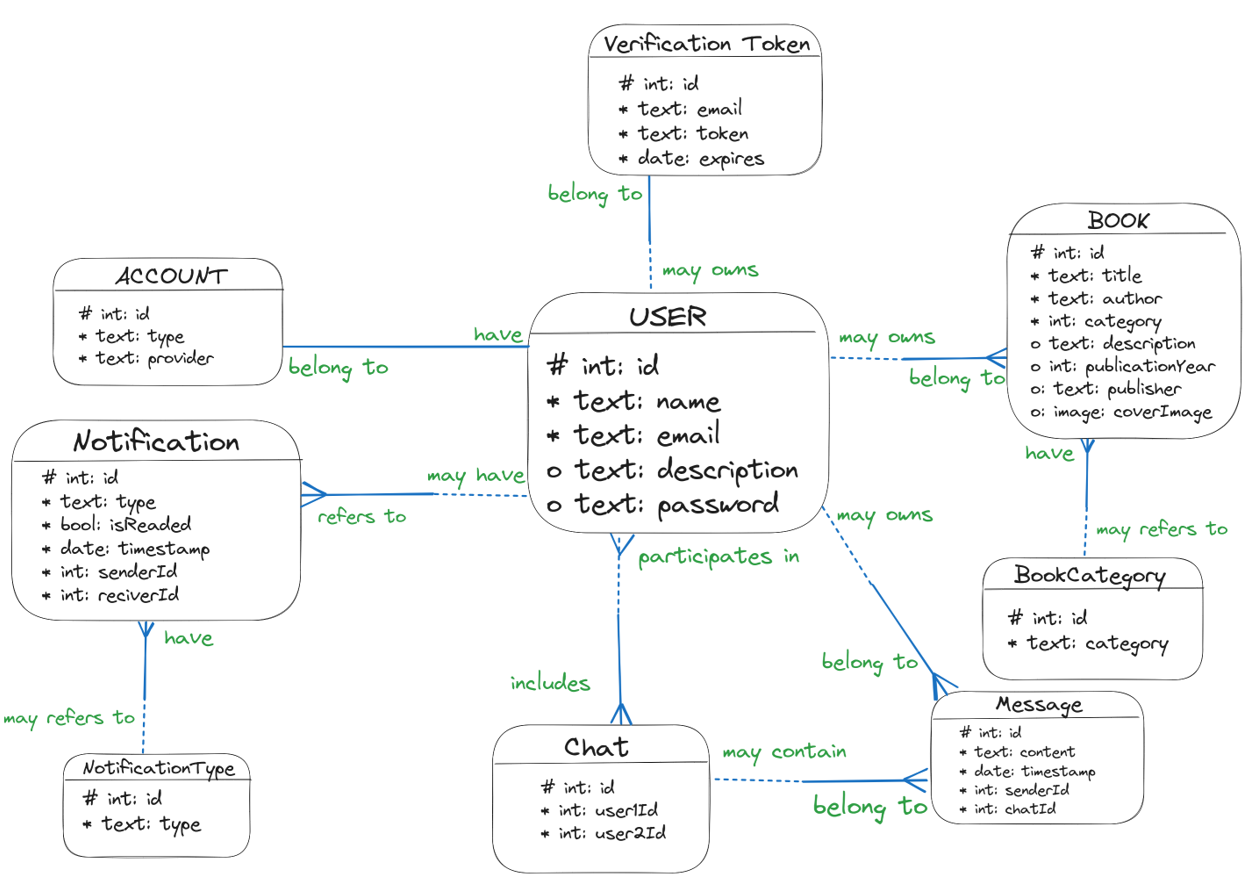
\includegraphics[width=17cm]{figures/diagramERD.png}
	\caption{Diagram ERD}
\end{figure}

\begin{figure}[h!]
	\centering
	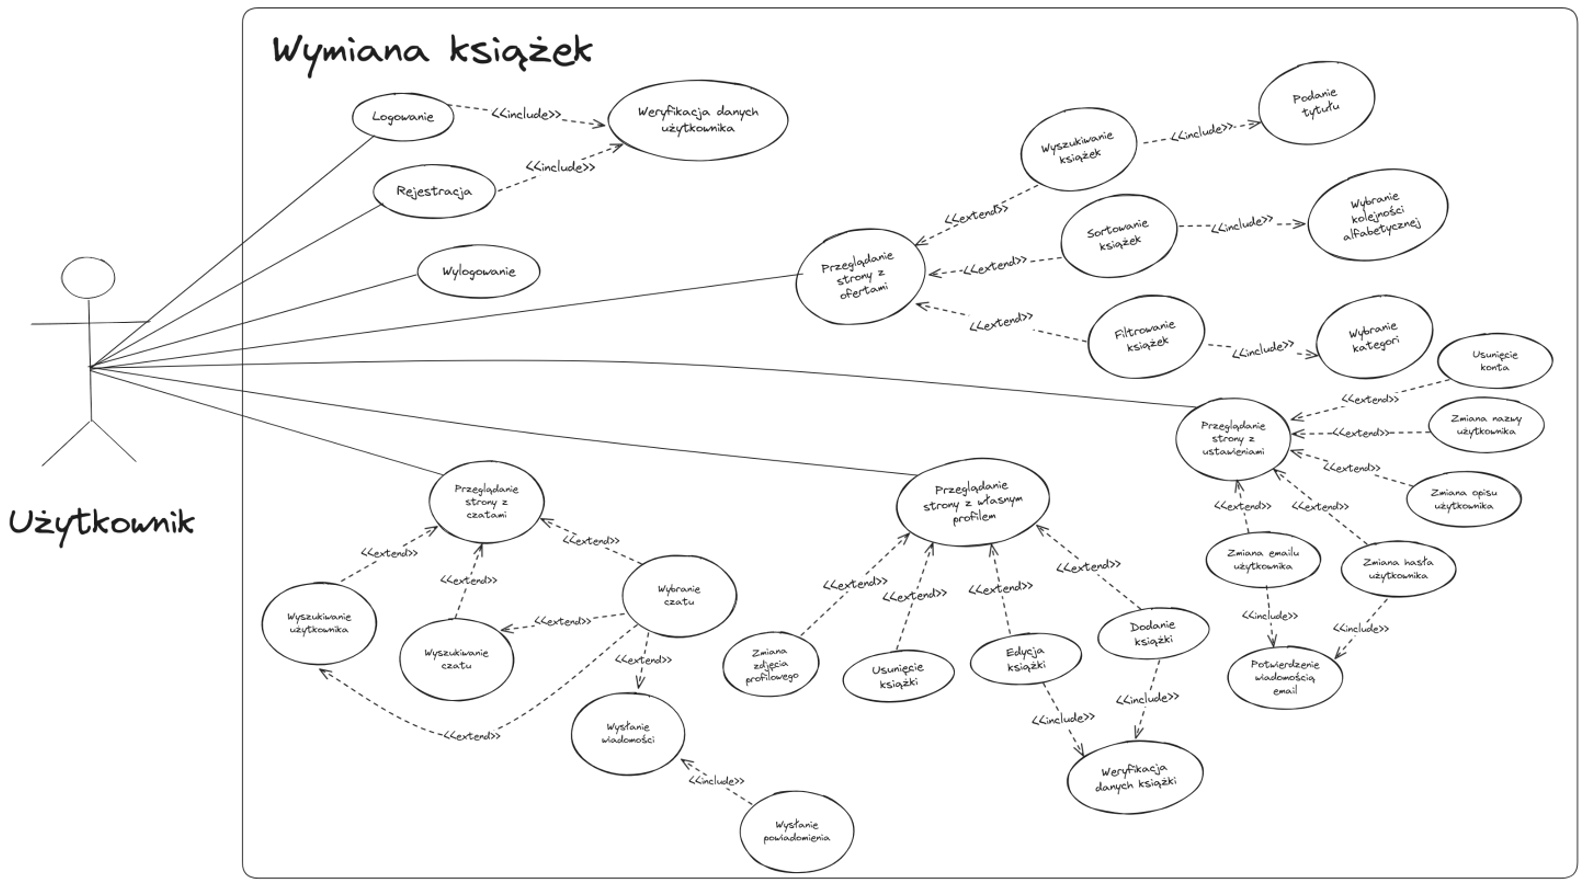
\includegraphics[width=18cm]{figures/diagramUCD.png}
	\caption{Diagram UCD}
\end{figure}

\begin{figure}[h!]
	\centering
	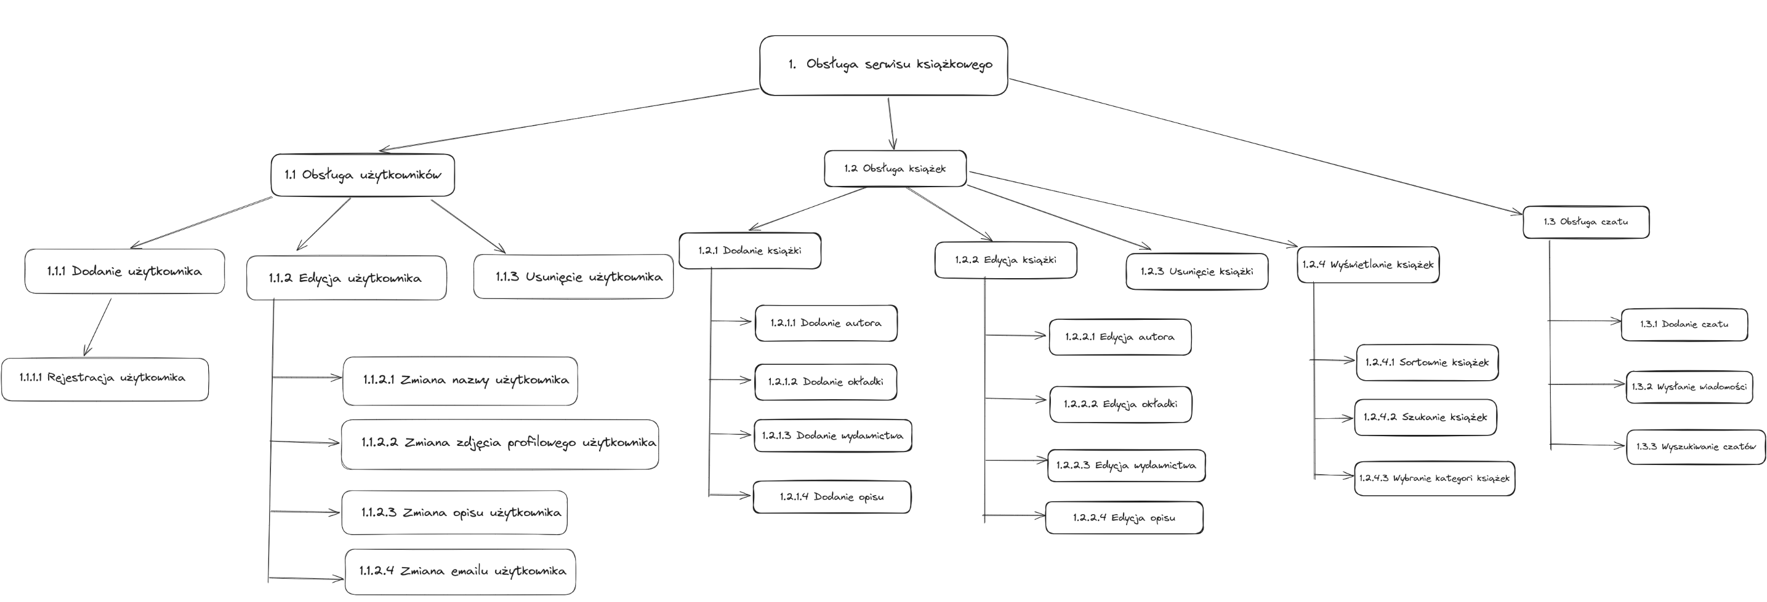
\includegraphics[width=18cm]{figures/diagramFHD.png}
	\caption{Diagram FHD}
\end{figure}

\clearpage
\section{Wygląd strony internetowej}


\begin{figure}[h!]
	\centering
	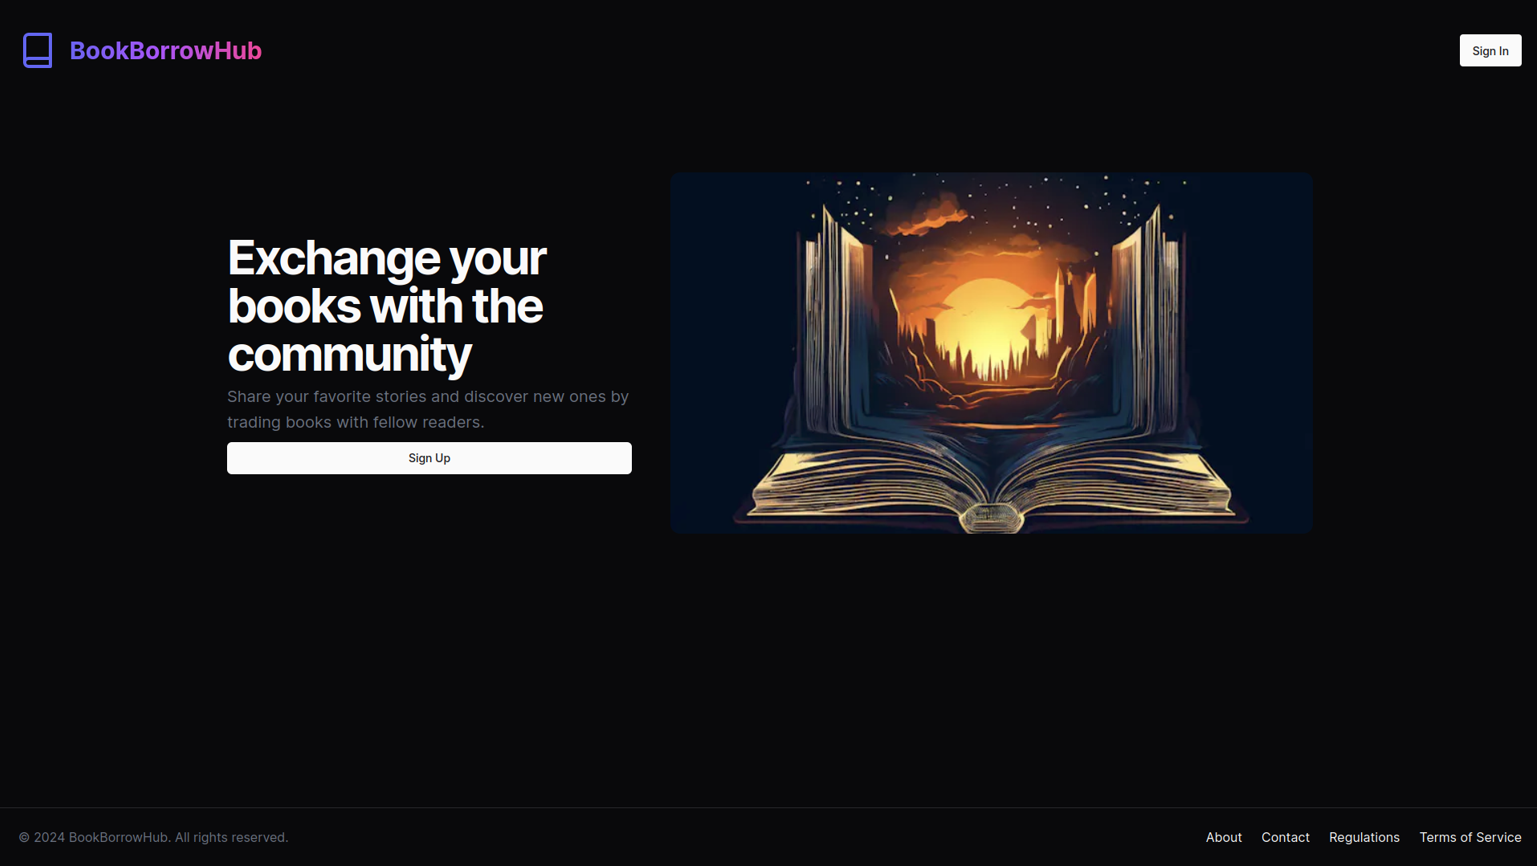
\includegraphics[width=17.5cm]{figures/Obraz5.png}
	\caption{Strona główna}
\end{figure}
Strona główna "BookBorrowHub" prezentuje minimalistyczne, 
ciemne tło, na którym widoczne są jasne elementy tekstowe 
i graficzne. Centralnym elementem jest dynamiczna ilustracja otwartej książki, 
która ma zachęcać użytkowników do korzystania ze strony oraz przycisk "Sign Up" który służy do rejestracji.
W górnej części strony znajduje się przycisk "Sign In", który służy do logowania. 
Na dole strony umieszczone są linki do dodatkowych informacji: "About", "Contact", 
"Regulations" i "Terms of Service". 
Całość projektu jest nowoczesna i funkcjonalna, zachęcając użytkownika do interakcji z platformą.


\newpage
\begin{figure}[h!]
	\centering
	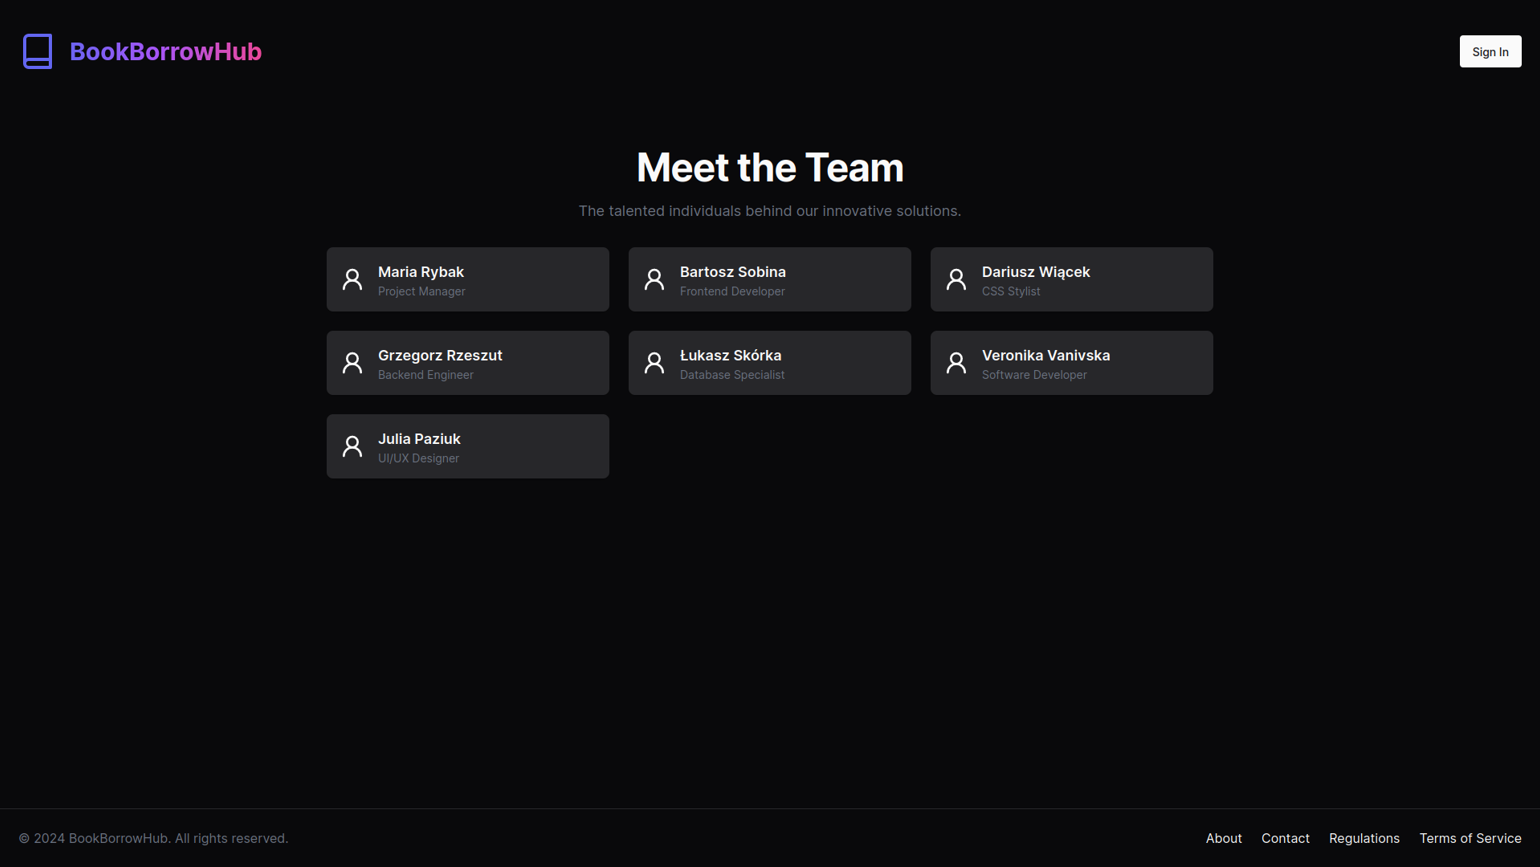
\includegraphics[width=17.5cm]{figures/Obraz6.png}
	\caption{Panel informacji o zespole developerów} 
\end{figure}
Widzimy tutaj zawartość zakładki 'About'. 
Przedstawia ona zespół developerów, 
który był odpowiedzialny za stworzenie strony wraz ze wszystkimi jej funkcjonalnościami.

\newpage
\begin{figure}[h!]
	\centering
	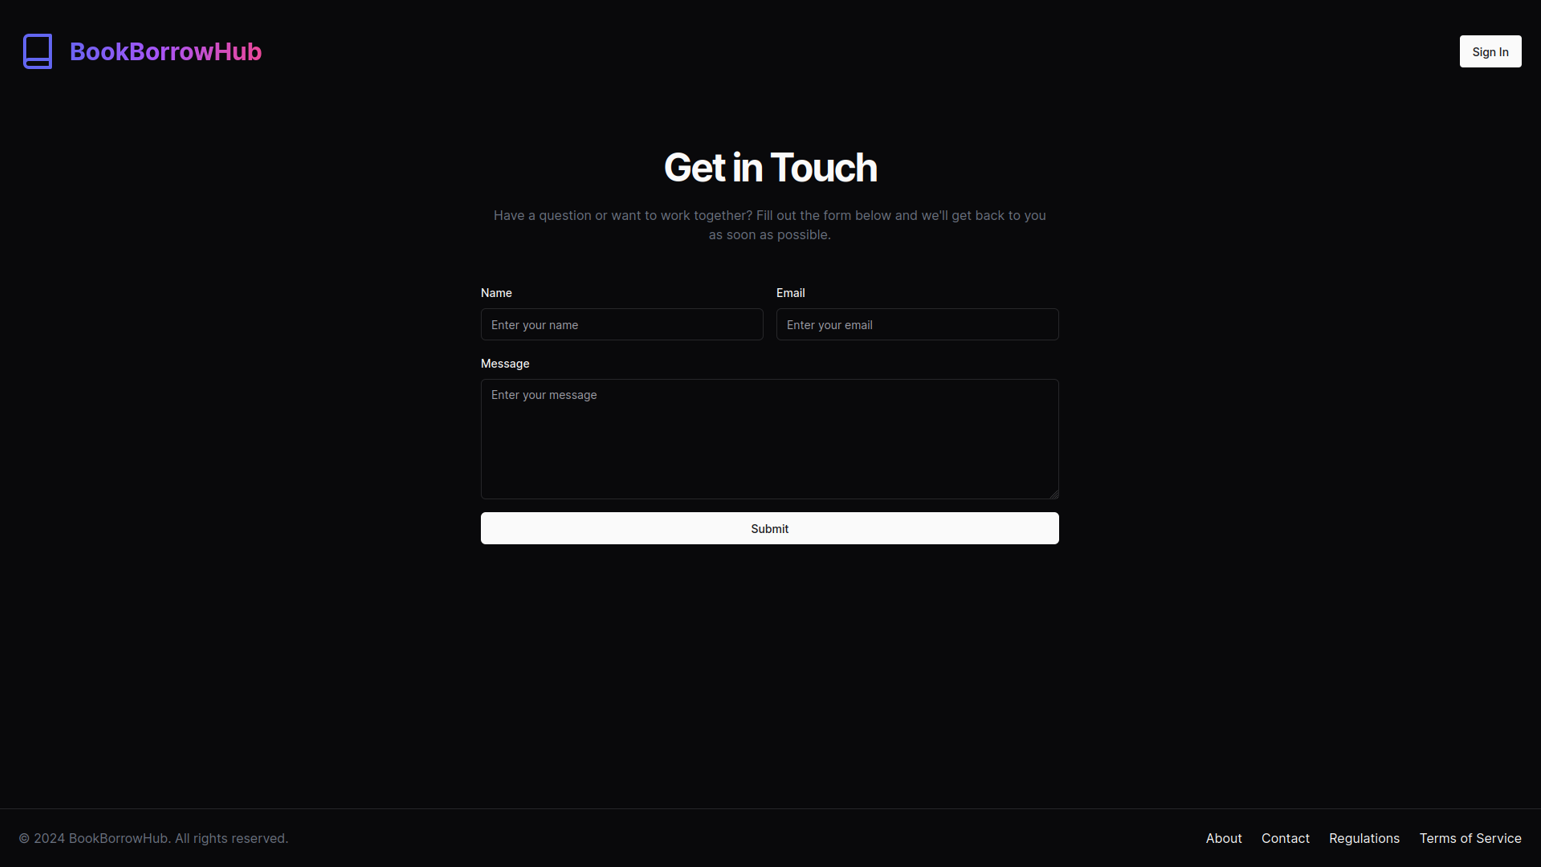
\includegraphics[width=17.5cm]{figures/Obraz7.png}
	\caption{Panel kontaktu z administracją strony}
\end{figure}
Na obrazie pokazany jest panel, 
dzięki któremu użytkownicy mogą skontaktować 
się z administracją strony w razie problemów z 
jej działaniem lub pytań. Aby się do niego dostać, 
trzeba kliknąć zakładkę 'Contact'. 
Aby wysłać wiadomość, trzeba podać swoją nazwę oraz e-mail.

\newpage
\begin{figure}[h!]
	\centering
	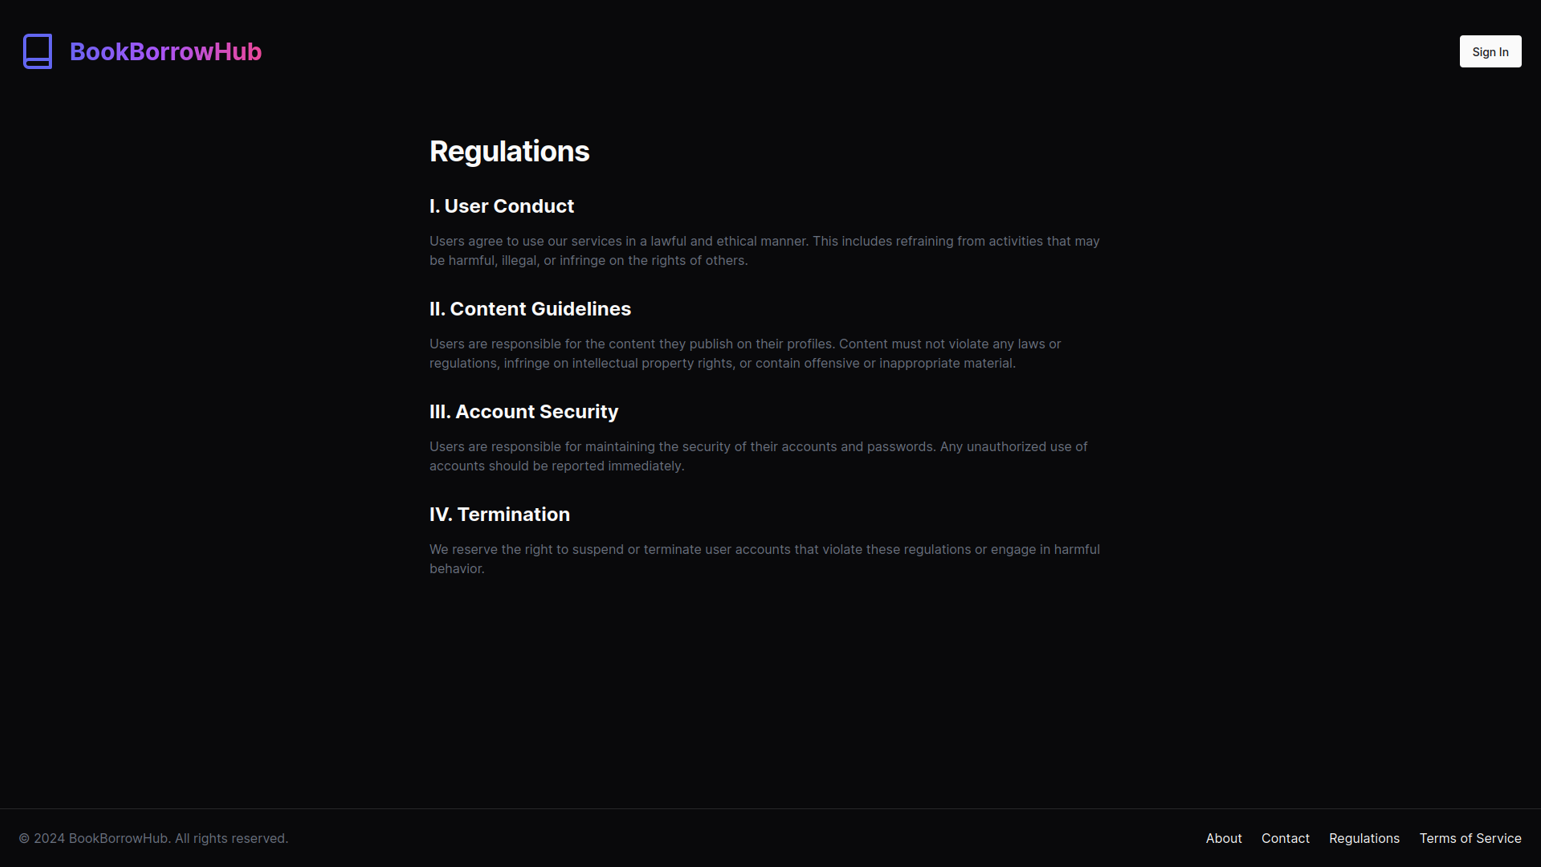
\includegraphics[width=17.5cm]{figures/Obraz8.png}
	\caption{Regulamin strony}
\end{figure}
Zrzut ekranu przedstawia regulamin, 
który obowiązuje wszystkich użytkowników strony. 
Osoba zakładająca konto na platformie automatycznie 
akceptuje warunki korzystania z niej. 
Aby wyświetlić tę stronę, należy kliknąć zakładkę 'Regulations'.

\newpage
\begin{figure}[h!]
	\centering
	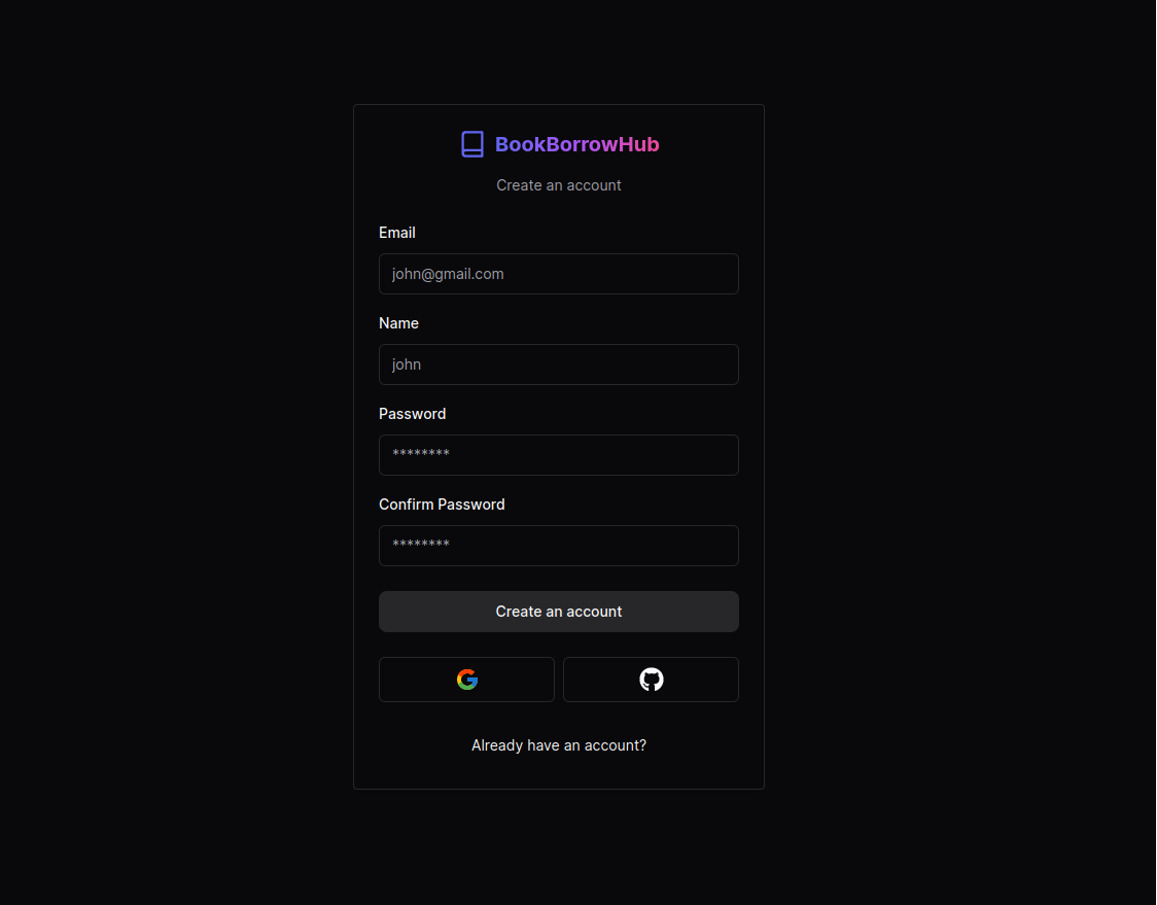
\includegraphics[width=17.5cm]{figures/Obraz9.png}
	\caption{Panel rejestracji}
\end{figure}
Aby założyć konto, wymagane jest podanie: e-mailu, 
nazwy użytkownika oraz hasła. 
Możliwe jest założenie konta poprzez 
konto Google lub GitHub. 
Jeśli użytkownik posiada już konto, 
może przejść do strony logowania, 
klikając przycisk 'Already have an account?'.

\newpage
\begin{figure}[h!]
	\centering
	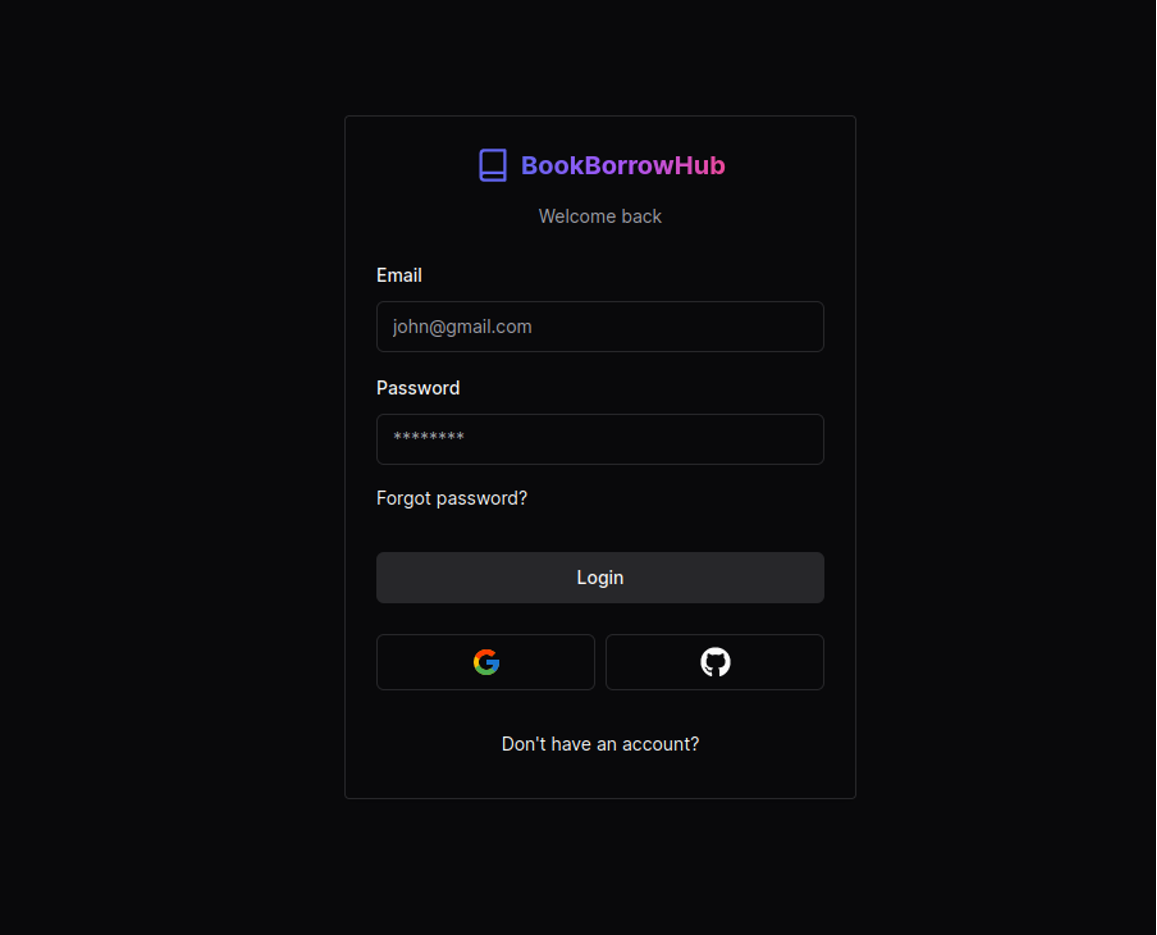
\includegraphics[width=17.5cm]{figures/Obraz10.png}
	\caption{Panel logowania}
\end{figure}
Aby się zalogować, trzeba podać e-mail oraz hasło. 
Istnieje możliwość zresetowania hasła i 
odzyskania dostępu do konta, klikając w opcję 
'Forgot password?'. Można również przejść do panelu rejestracji, 
klikając przycisk 'Don't have an account?'.

\newpage
\begin{figure}[h!]
	\centering
	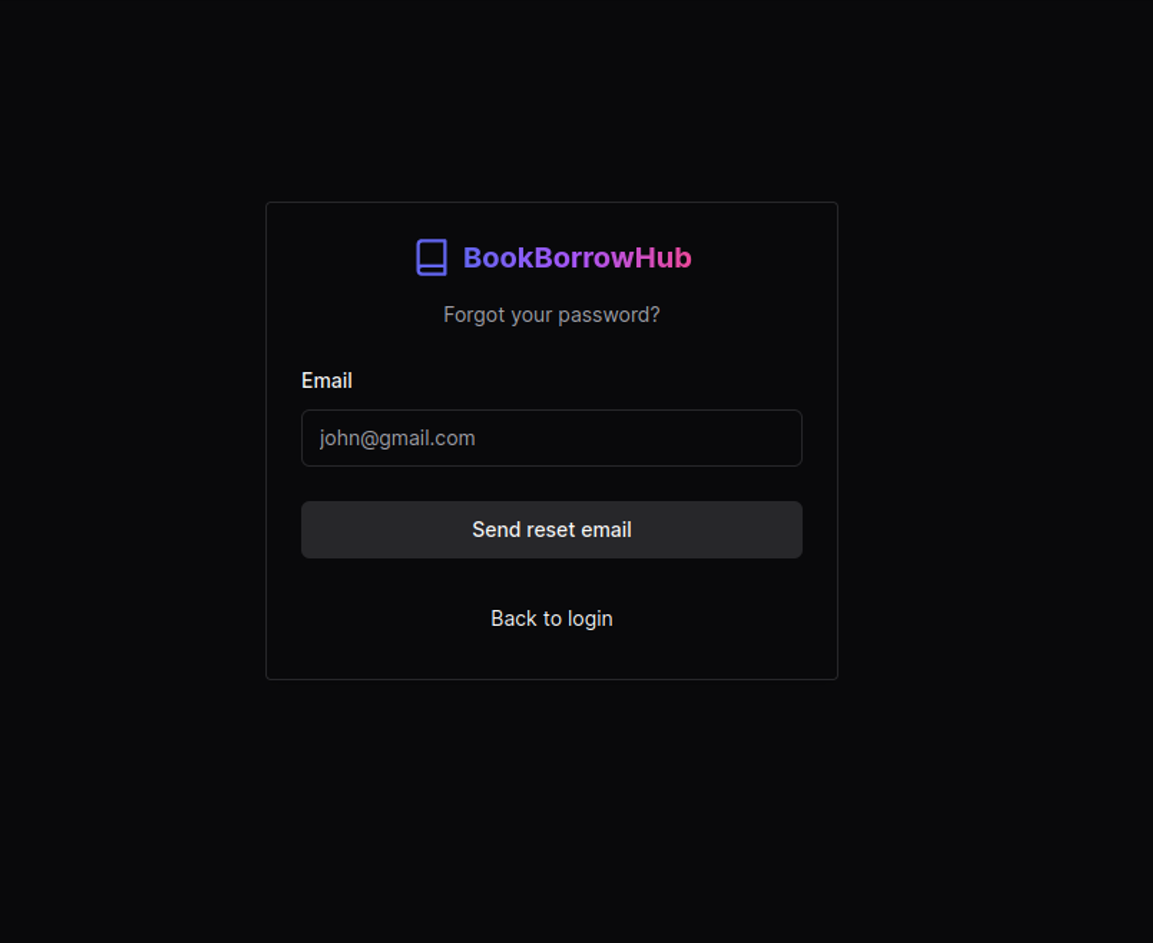
\includegraphics[width=17.5cm]{figures/Obraz11.png}
	\caption{Panel zmiany hasła}
\end{figure}
Aby zresetować hasło, 
należy podać e-mail, którym logujemy się do strony. 
Po zatwierdzeniu na skrzynkę pocztową 
zostanie wysłany link umożliwiający ustawienie nowego hasła.

\newpage
\begin{figure}[h!]
	\centering
	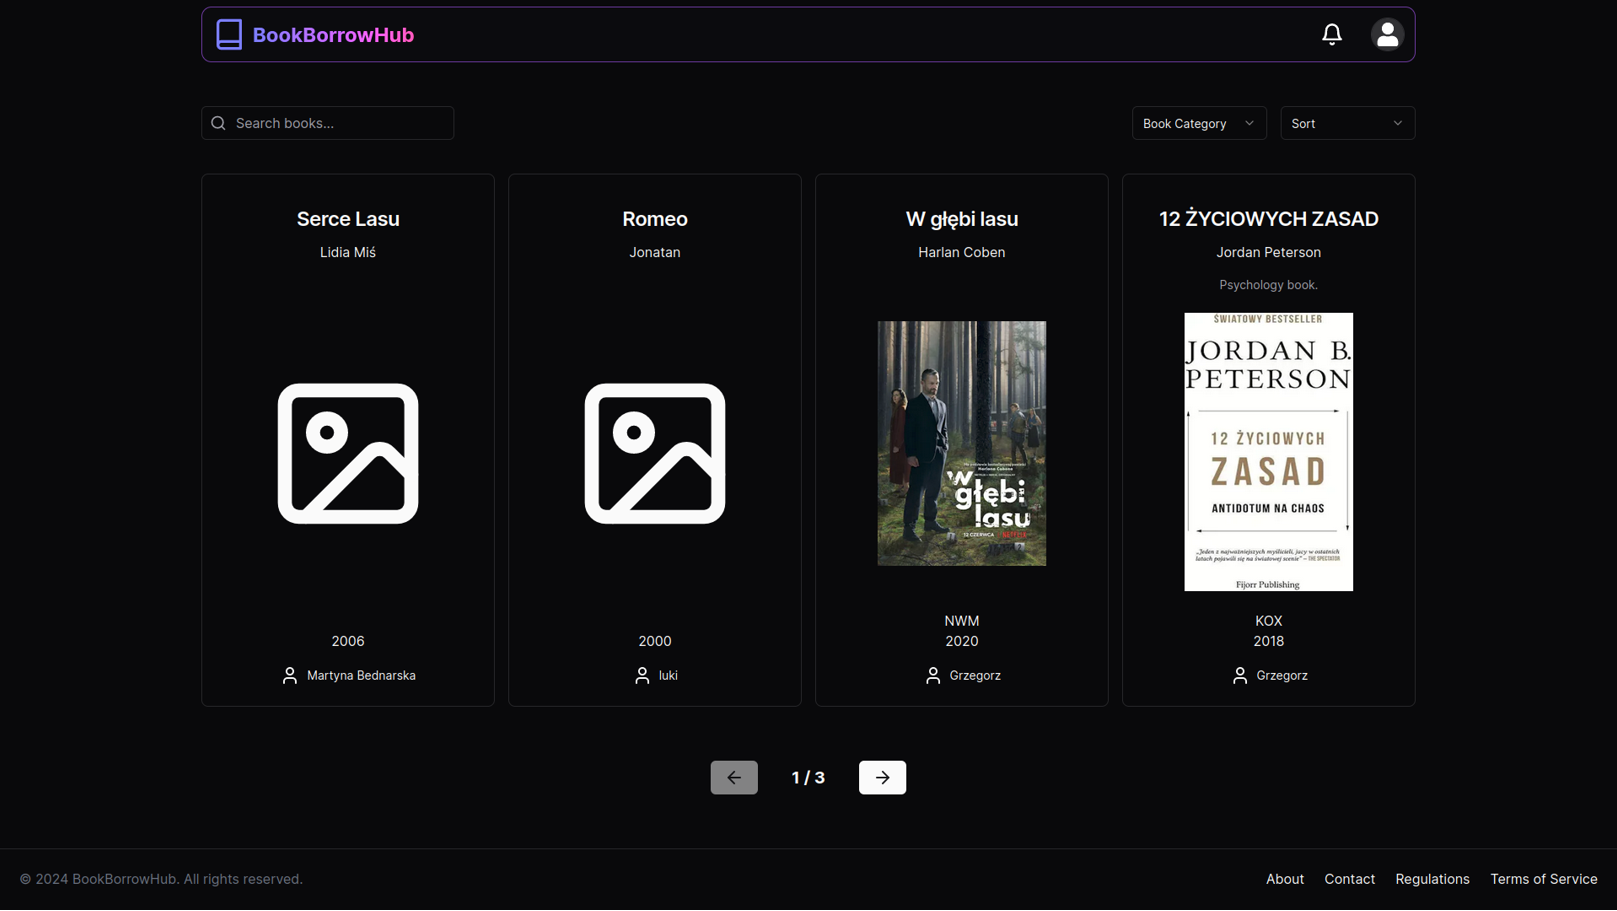
\includegraphics[width=17.5cm]{figures/Obraz12.png}
	\caption{Panel ofert wymiany użytkowników strony}
\end{figure}
Strona wyświetla oferty wymiany książek wszystkich użytkowników. 
Można posortować wyświetlane pozycje oraz wybrać kategorię książek, 
która nas interesuje. Możliwe jest również wyszukanie książki po nazwie.

\newpage
\begin{figure}[h!]
	\centering
	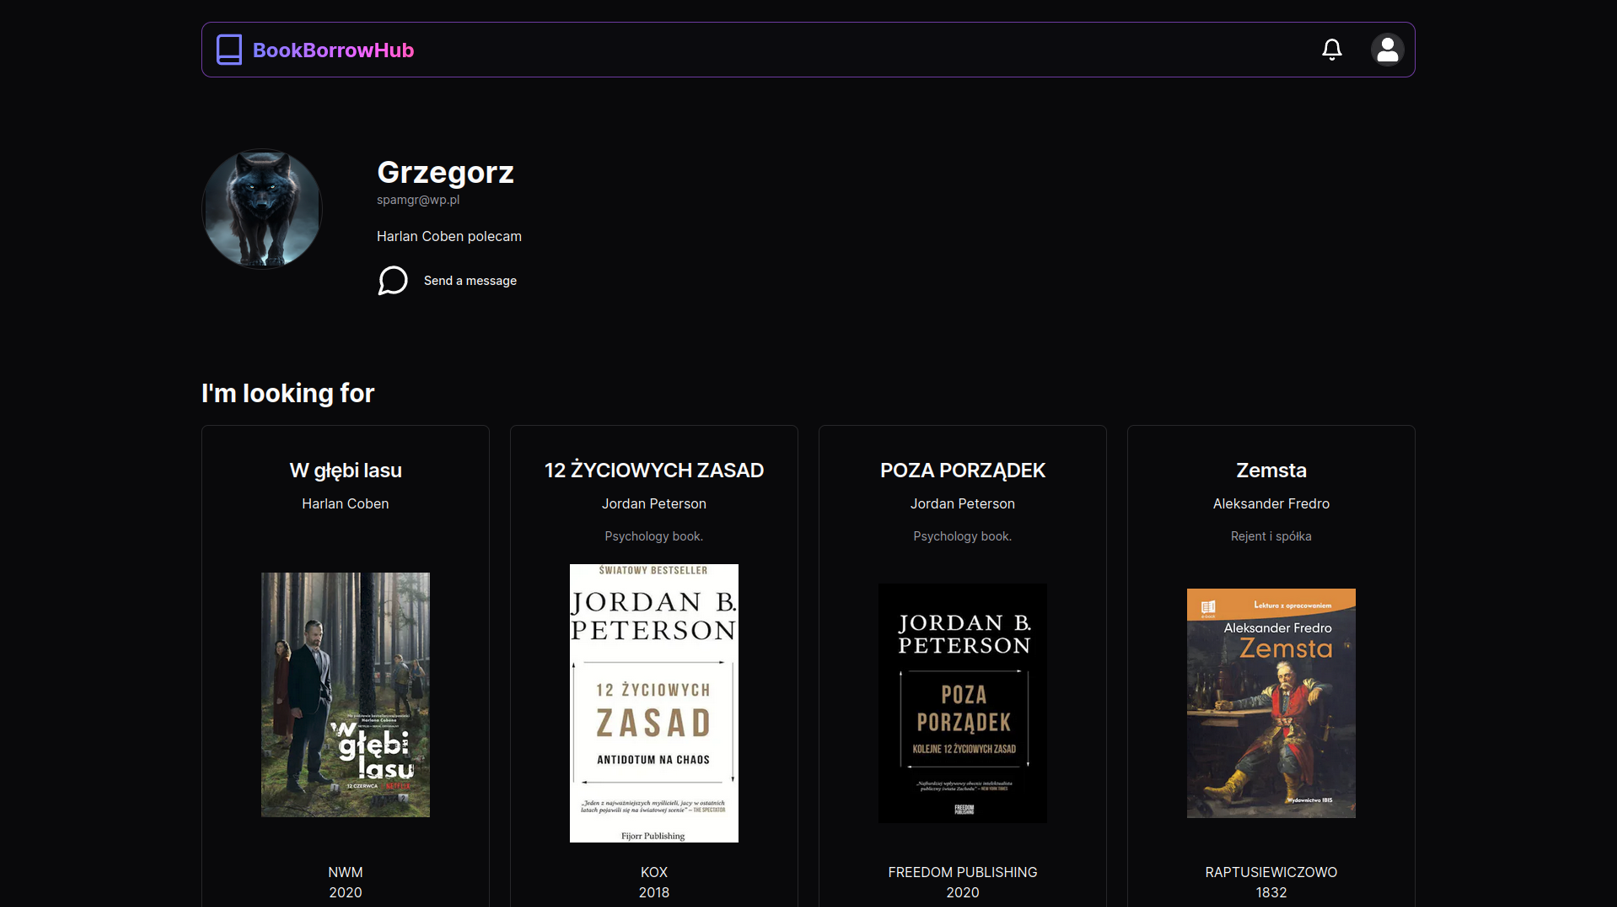
\includegraphics[width=17.5cm]{figures/Obraz13.png}
	\caption{Panel ofert wymiany innego użytkownika}
\end{figure}
Strona domowa użytkownika wyświetla jego zdjęcie profilowe, 
e-mail oraz informację, jaką użytkownik chce podać o sobie. 
Jest również możliwość rozpoczęcia z nim konwersacji. 
Pod danymi użytkownika wyświetlane są pozycje, 
które chce on wymienić, oraz pozycje, których szuka.

\newpage
\begin{figure}[h!]
	\centering
	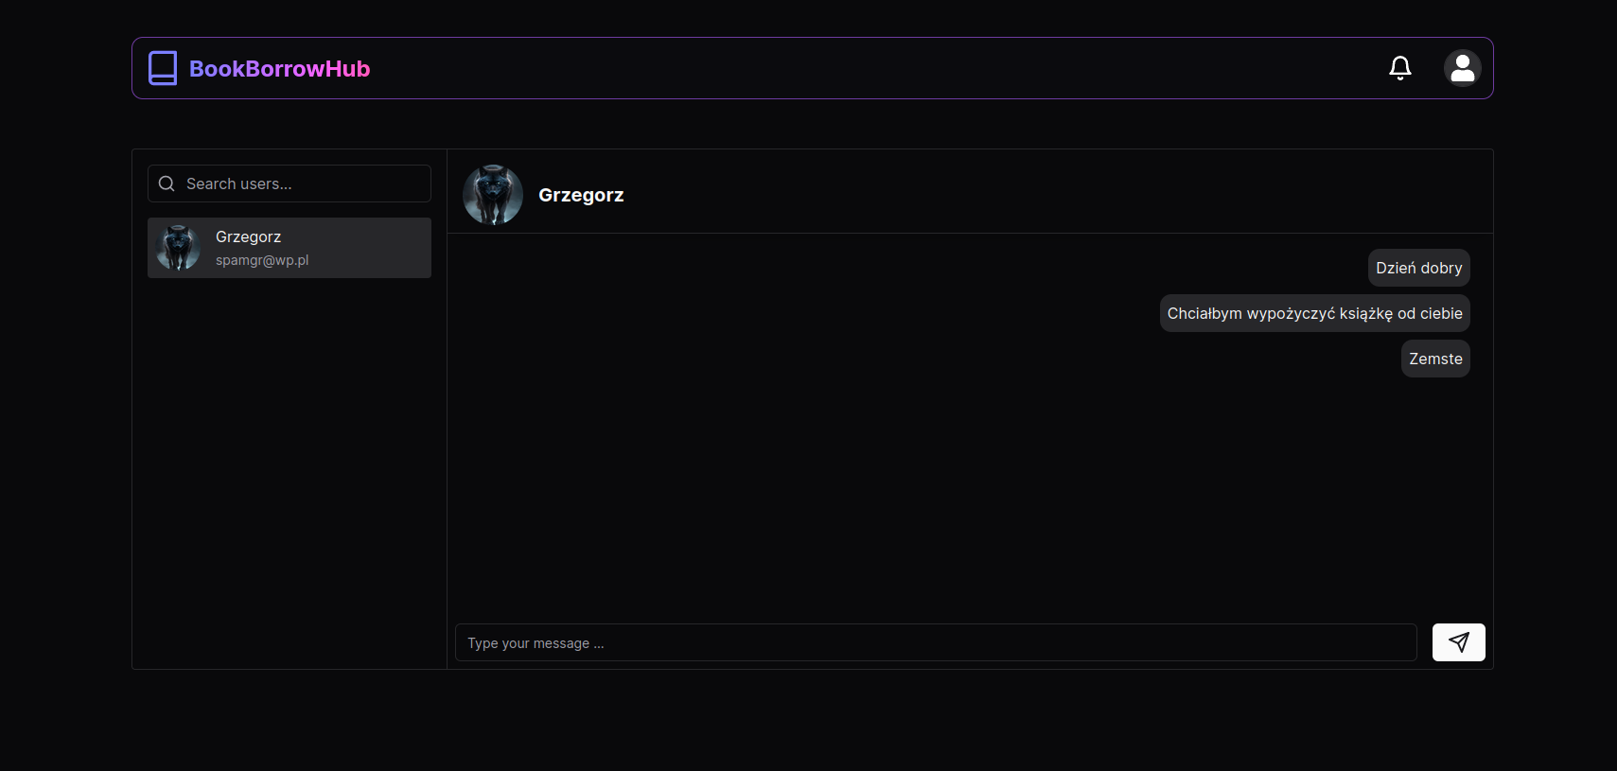
\includegraphics[width=17.5cm]{figures/Obraz14.png}
	\caption{Panel czatów z innymi użytkownikami}
\end{figure}
Panel rozmów daje możliwość znalezienia użytkownika, 
z którym chcemy rozpocząć konwersację lub 
z którym już prowadziliśmy rozmowę. 
Wybieramy osobę i możemy przejrzeć historię konwersacji lub wysłać nową wiadomość.

\newpage
\begin{figure}[h!]
	\centering
	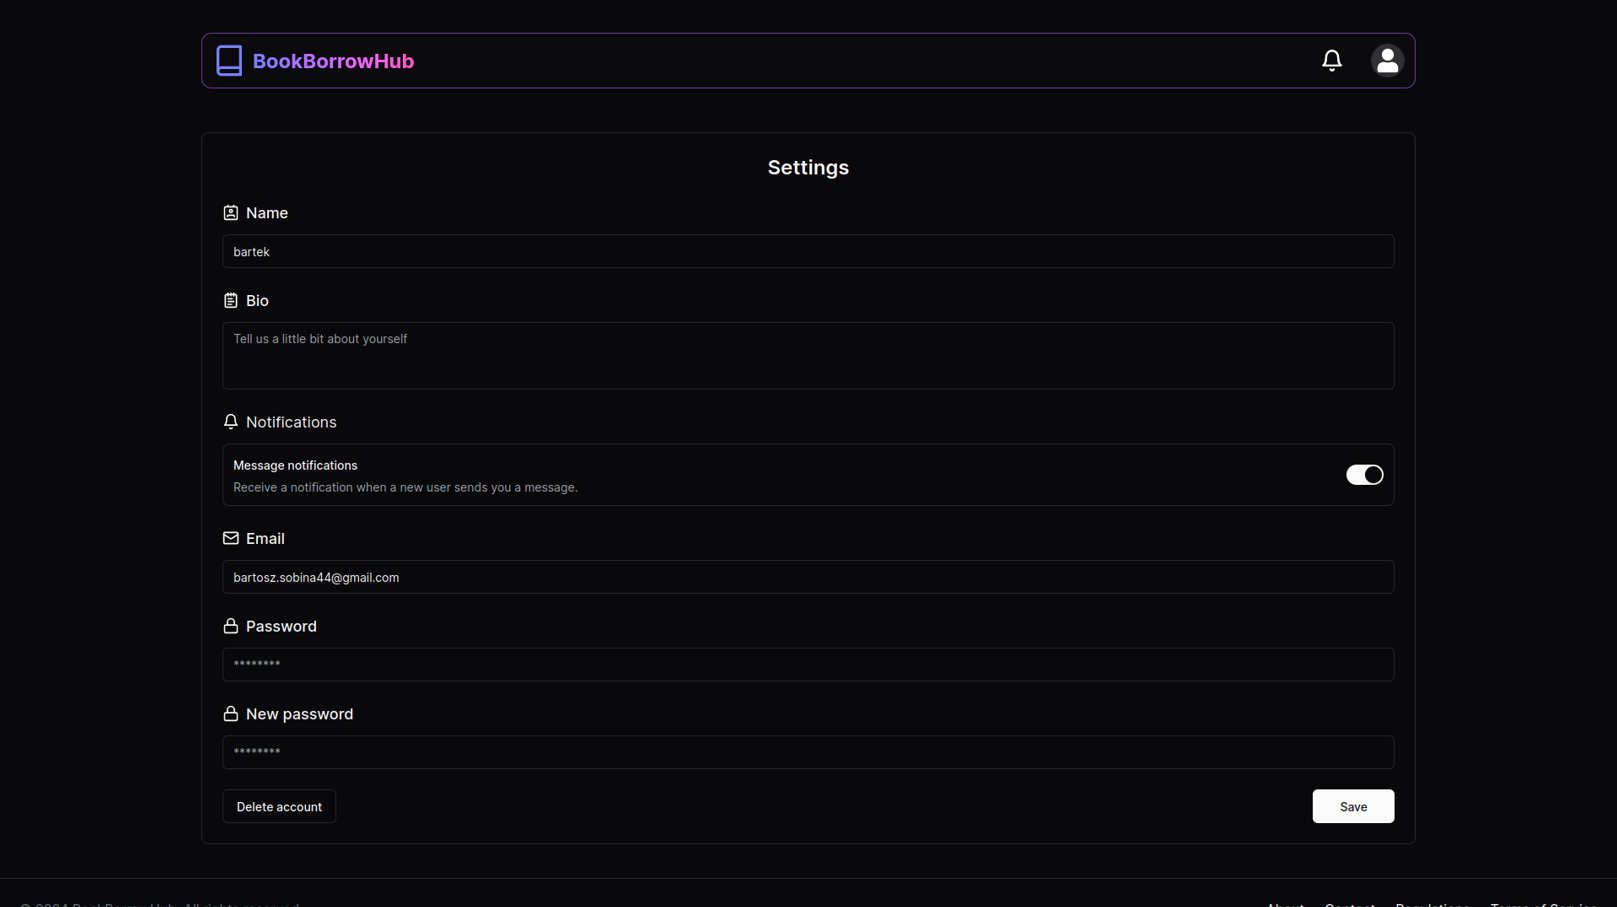
\includegraphics[width=17.5cm]{figures/Obraz15.png}
	\caption{Panel ustawień użytkownika}
\end{figure}
W panelu ustawień użytkownika można ustawić informacje 
takie jak nazwa i bio, a także wyłączyć powiadomienia, 
zmienić adres e-mail oraz hasło. 
Jest możliwość usunięcia swojego konta na platformie.

\newpage
\begin{figure}[h!]
	\centering
	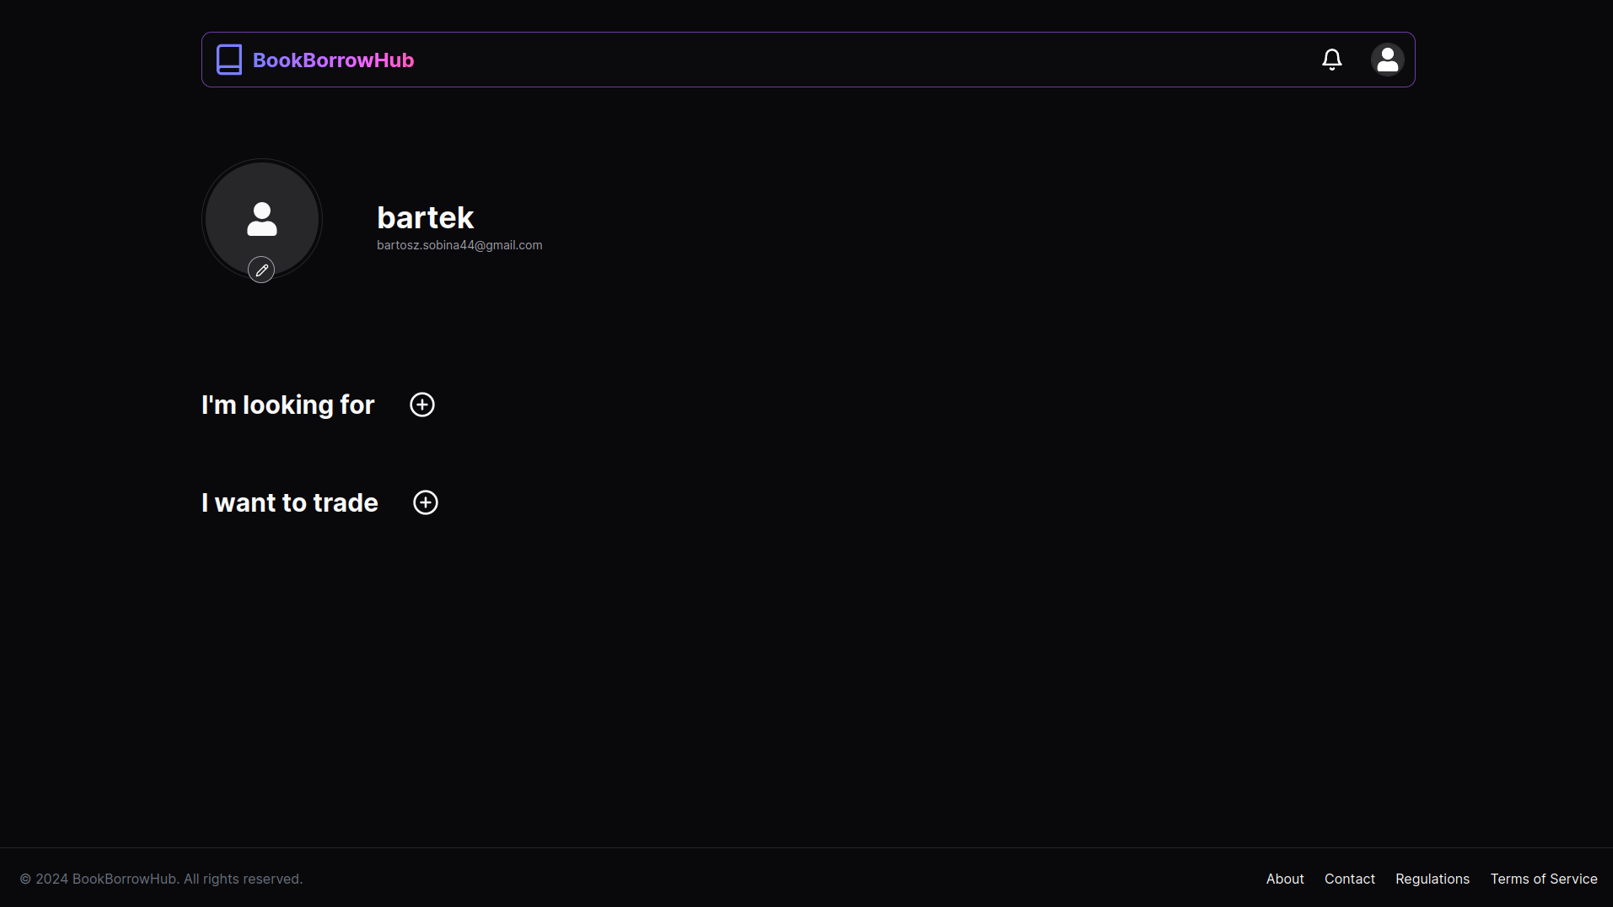
\includegraphics[width=17.5cm]{figures/Obraz16.png}
	\caption{Panel profilu użytkownika}
\end{figure}
Tutaj widzimy panel profilu, 
w którym mamy możliwość zmiany zdjęcia profilowego oraz dodania, 
edytowania i usunięcia ofert wymiany zalogowanego użytkownika.

\newpage
\begin{figure}[h!]
	\centering
	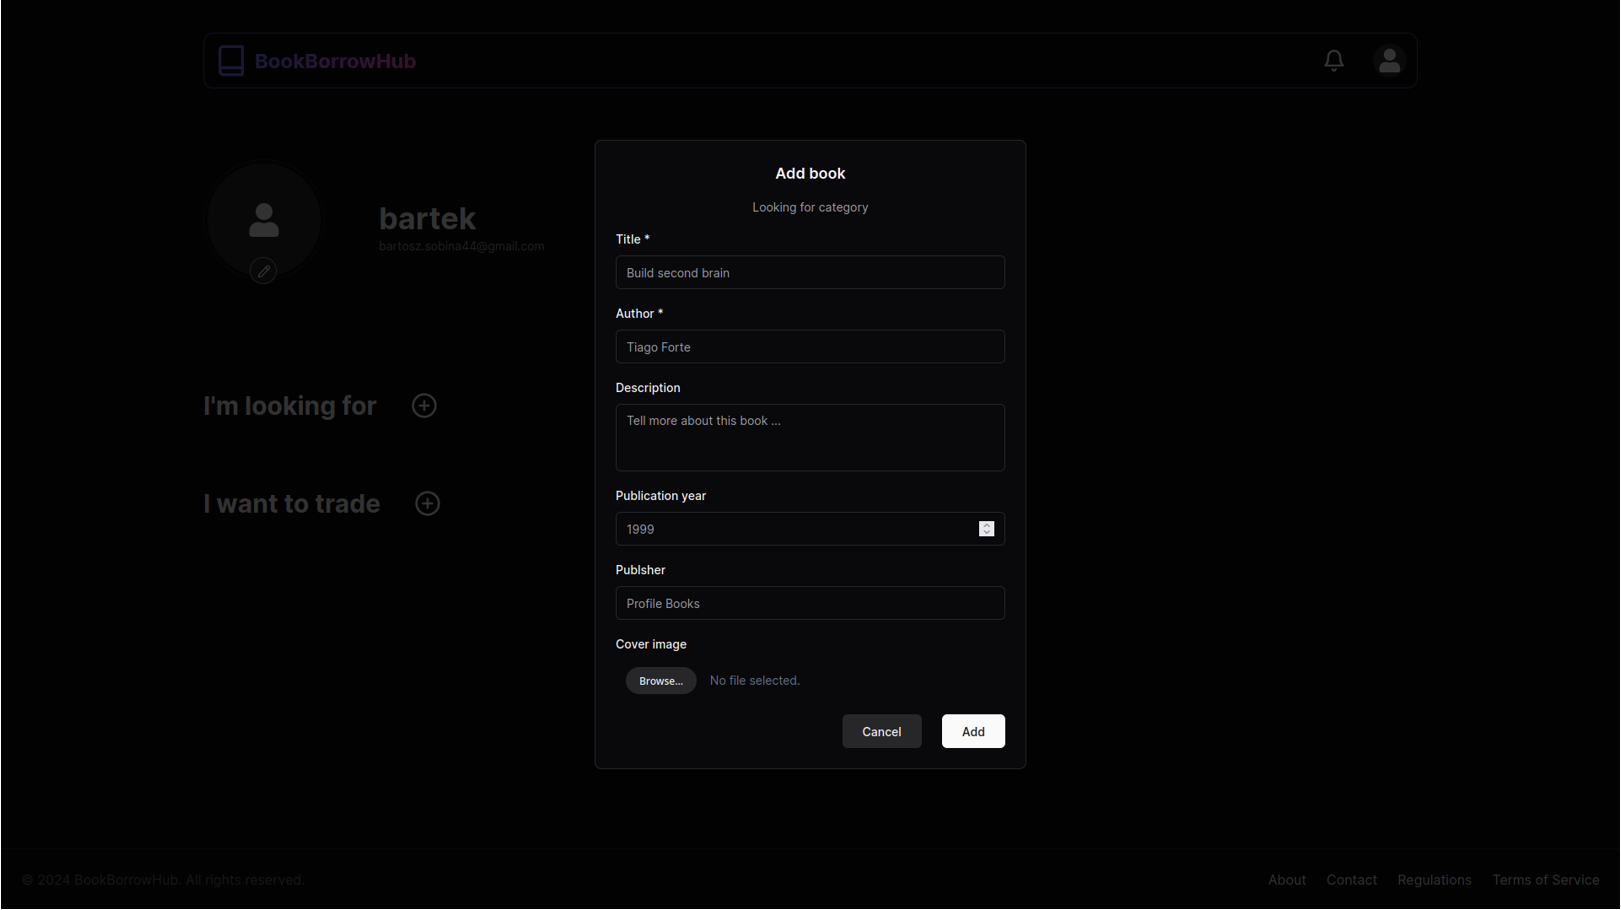
\includegraphics[width=17.5cm]{figures/Obraz17.png}
	\caption{Panel dodania ogłoszenia/książki}
\end{figure}
Chcąc dodać ofertę wymiany, 
trzeba podać informacje takie jak: tytuł, autor, opis, 
rok wydania, wydawnictwo oraz zdjęcie. 
Po dodaniu ogłoszenia będzie ono widoczne 
na stronie ze wszystkimi ofertami oraz na profilu użytkownika.

\newpage
\begin{figure}[h!]
	\centering
	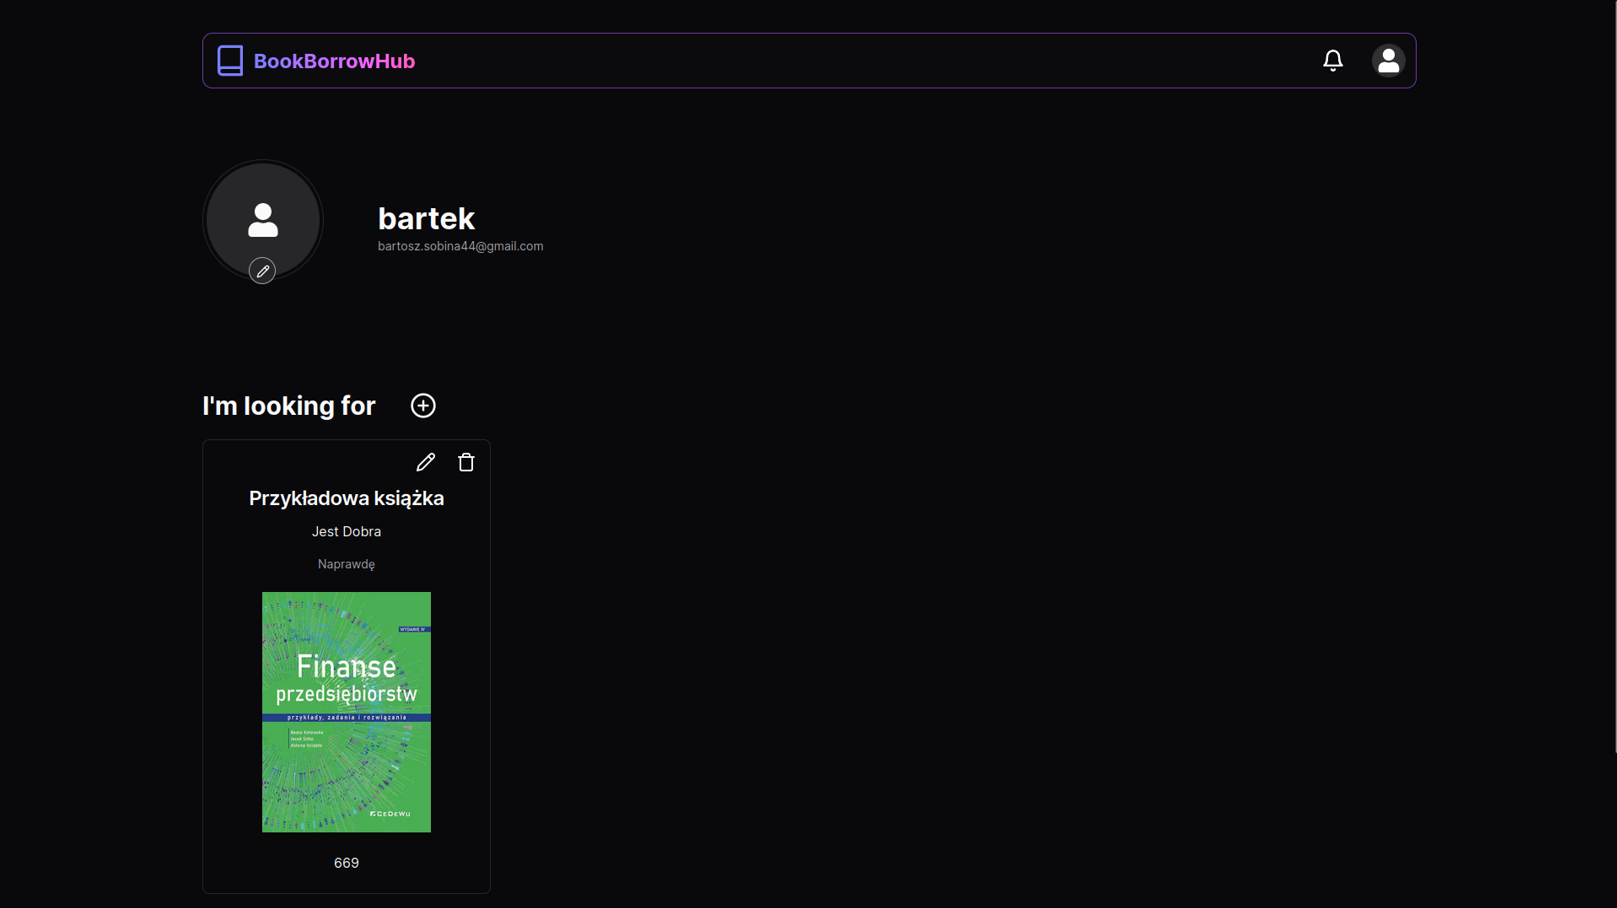
\includegraphics[width=17.5cm]{figures/Obraz18.png}
	\caption{Panel profilu użytkownika z dodanymi książkami}
\end{figure}
Dodane książki można na swoim profilu edytować lub usunąć.

\newpage
\begin{figure}[h!]
	\centering
	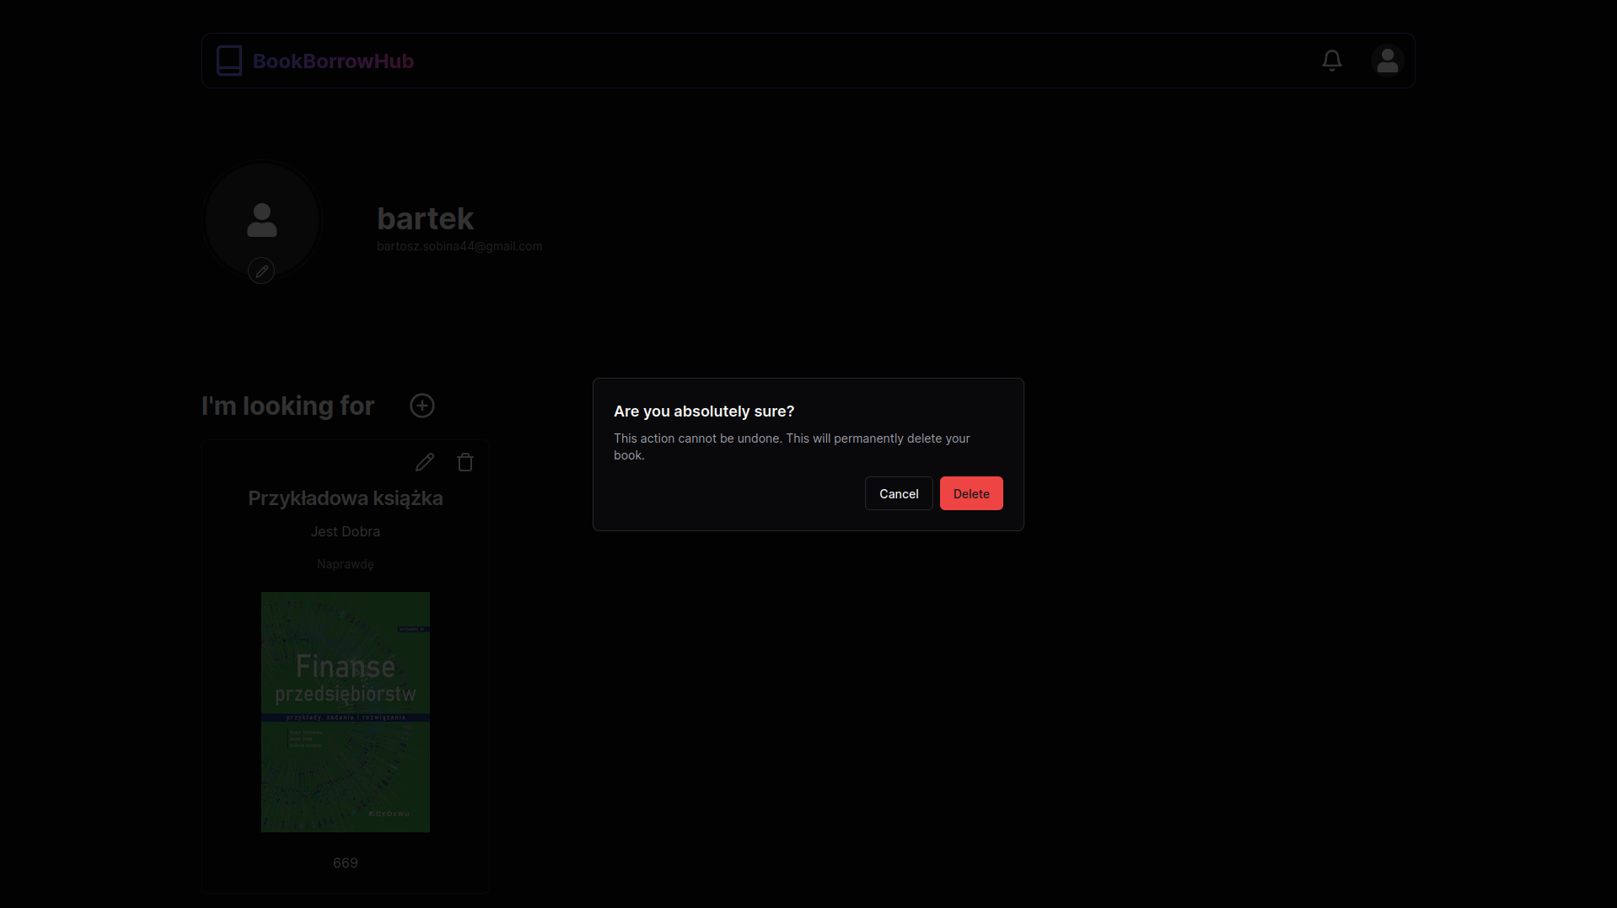
\includegraphics[width=17.5cm]{figures/Obraz19.png}
	\caption{Okienko usunięcia pozycji ze swoich ofert wymiany}
\end{figure}
Usunięcie swojej pozycji należy dodatkowo potwierdzić w oknie dialogowym.

\newpage
\begin{figure}[h!]
	\centering
	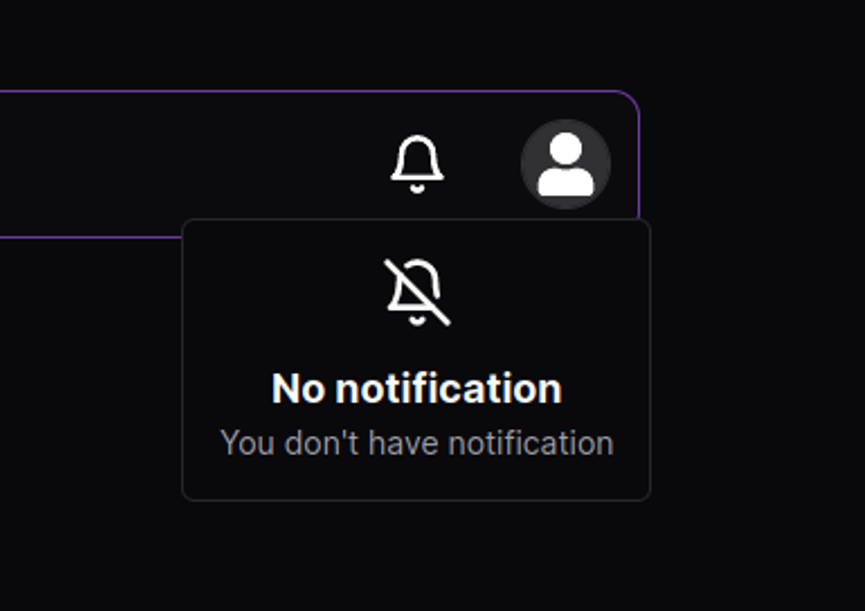
\includegraphics[width=17.5cm]{figures/Obraz20.png}
	\caption{Widget powiadomień (brak powiadomień)}
\end{figure}


\newpage
\begin{figure}[h!]
	\centering
	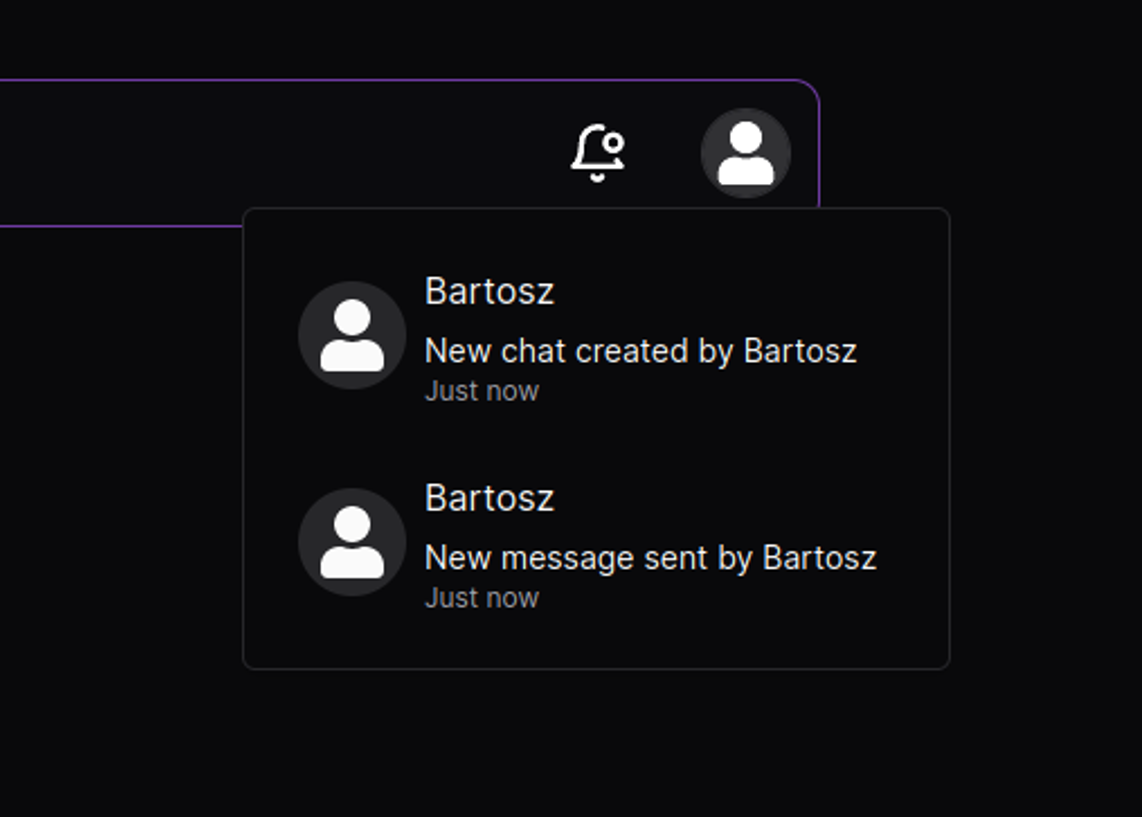
\includegraphics[width=17.5cm]{figures/Obraz21.png}
	\caption{Wideget powiadomień (kilka powidomień)}
\end{figure}
Powiadomienia o nowych konwersacjach wyświetlane 
są w prawym górnym rogu strony. 
Są przedstawiane w taki sposób, jak widać na obrazie.

\end{document}
